\documentclass[11pt, a4paper]{article}
% \usepackage[T1]{fontenc}
\usepackage[utf8]{inputenc}
\usepackage{listings}
\usepackage[margin=1.0in]{geometry}
\usepackage{color}
\usepackage{graphicx}
\usepackage{tabularx}
\usepackage{url} 

\title{Rock the net}
\author{Elias Frantar}
\author{Samuel Schmidt}
\author{Nikolaus Schrack}
\author{Gary Ye}
\date{\today{}, Wien}
\begin{document}

\lstset{ %
  backgroundcolor=\color{white},   % choose the background color; you must add \usepackage{color} or \usepackage{xcolor}
  basicstyle=\footnotesize,        % the size of the fonts that are used for the code
  breakatwhitespace=false,         % sets if automatic breaks should only happen at whitespace
  breaklines=true,                 % sets automatic line breaking
  captionpos=b,                    % sets the caption-position to bottom
% commentstyle=\color{mygreen},    % comment style
  deletekeywords={...},            % if you want to delete keywords from the given language
  escapeinside={\%*}{*)},          % if you want to add LaTeX within your code
  extendedchars=true,              % lets you use non-ASCII characters; for 8-bits encodings only, does not work with UTF-8
% frame=single,                    % adds a frame around the code
  keepspaces=true,                 % keeps spaces in text, useful for keeping indentation of code (possibly needs columns=flexible)
% keywordstyle=\color{blue},       % keyword style
% language=bash,                   % the language of the code
  morekeywords={*,...},            % if you want to add more keywords to the set
  numbers=left,                    % where to put the line-numbers; possible values are (none, left, right)
  numbersep=5pt,                   % how far the line-numbers are from the code
% numberstyle=\tiny\color{mygray}, % the style that is used for the line-numbers
  rulecolor=\color{black},         % if not set, the frame-color may be changed on line-breaks within not-black text (e.g. comments (green here))
  showspaces=false,                % show spaces everywhere adding particular underscores; it overrides 'showstringspaces'
  showstringspaces=false,          % underline spaces within strings only
  showtabs=false,                  % show tabs within strings adding particular underscores
  stepnumber=1,                    % the step between two line-numbers. If it's 1, each line will be numbered
% stringstyle=\color{mymauve},     % string literal style
  tabsize=2,                       % sets default tabsize to 2 spaces
  title=\lstname                   % show the filename of files included with \lstinputlisting; also try caption instead of title
}


\maketitle
\newpage
\tableofcontents
\newpage

\section{Task description}
% TODO
\section{Design}
% TODO
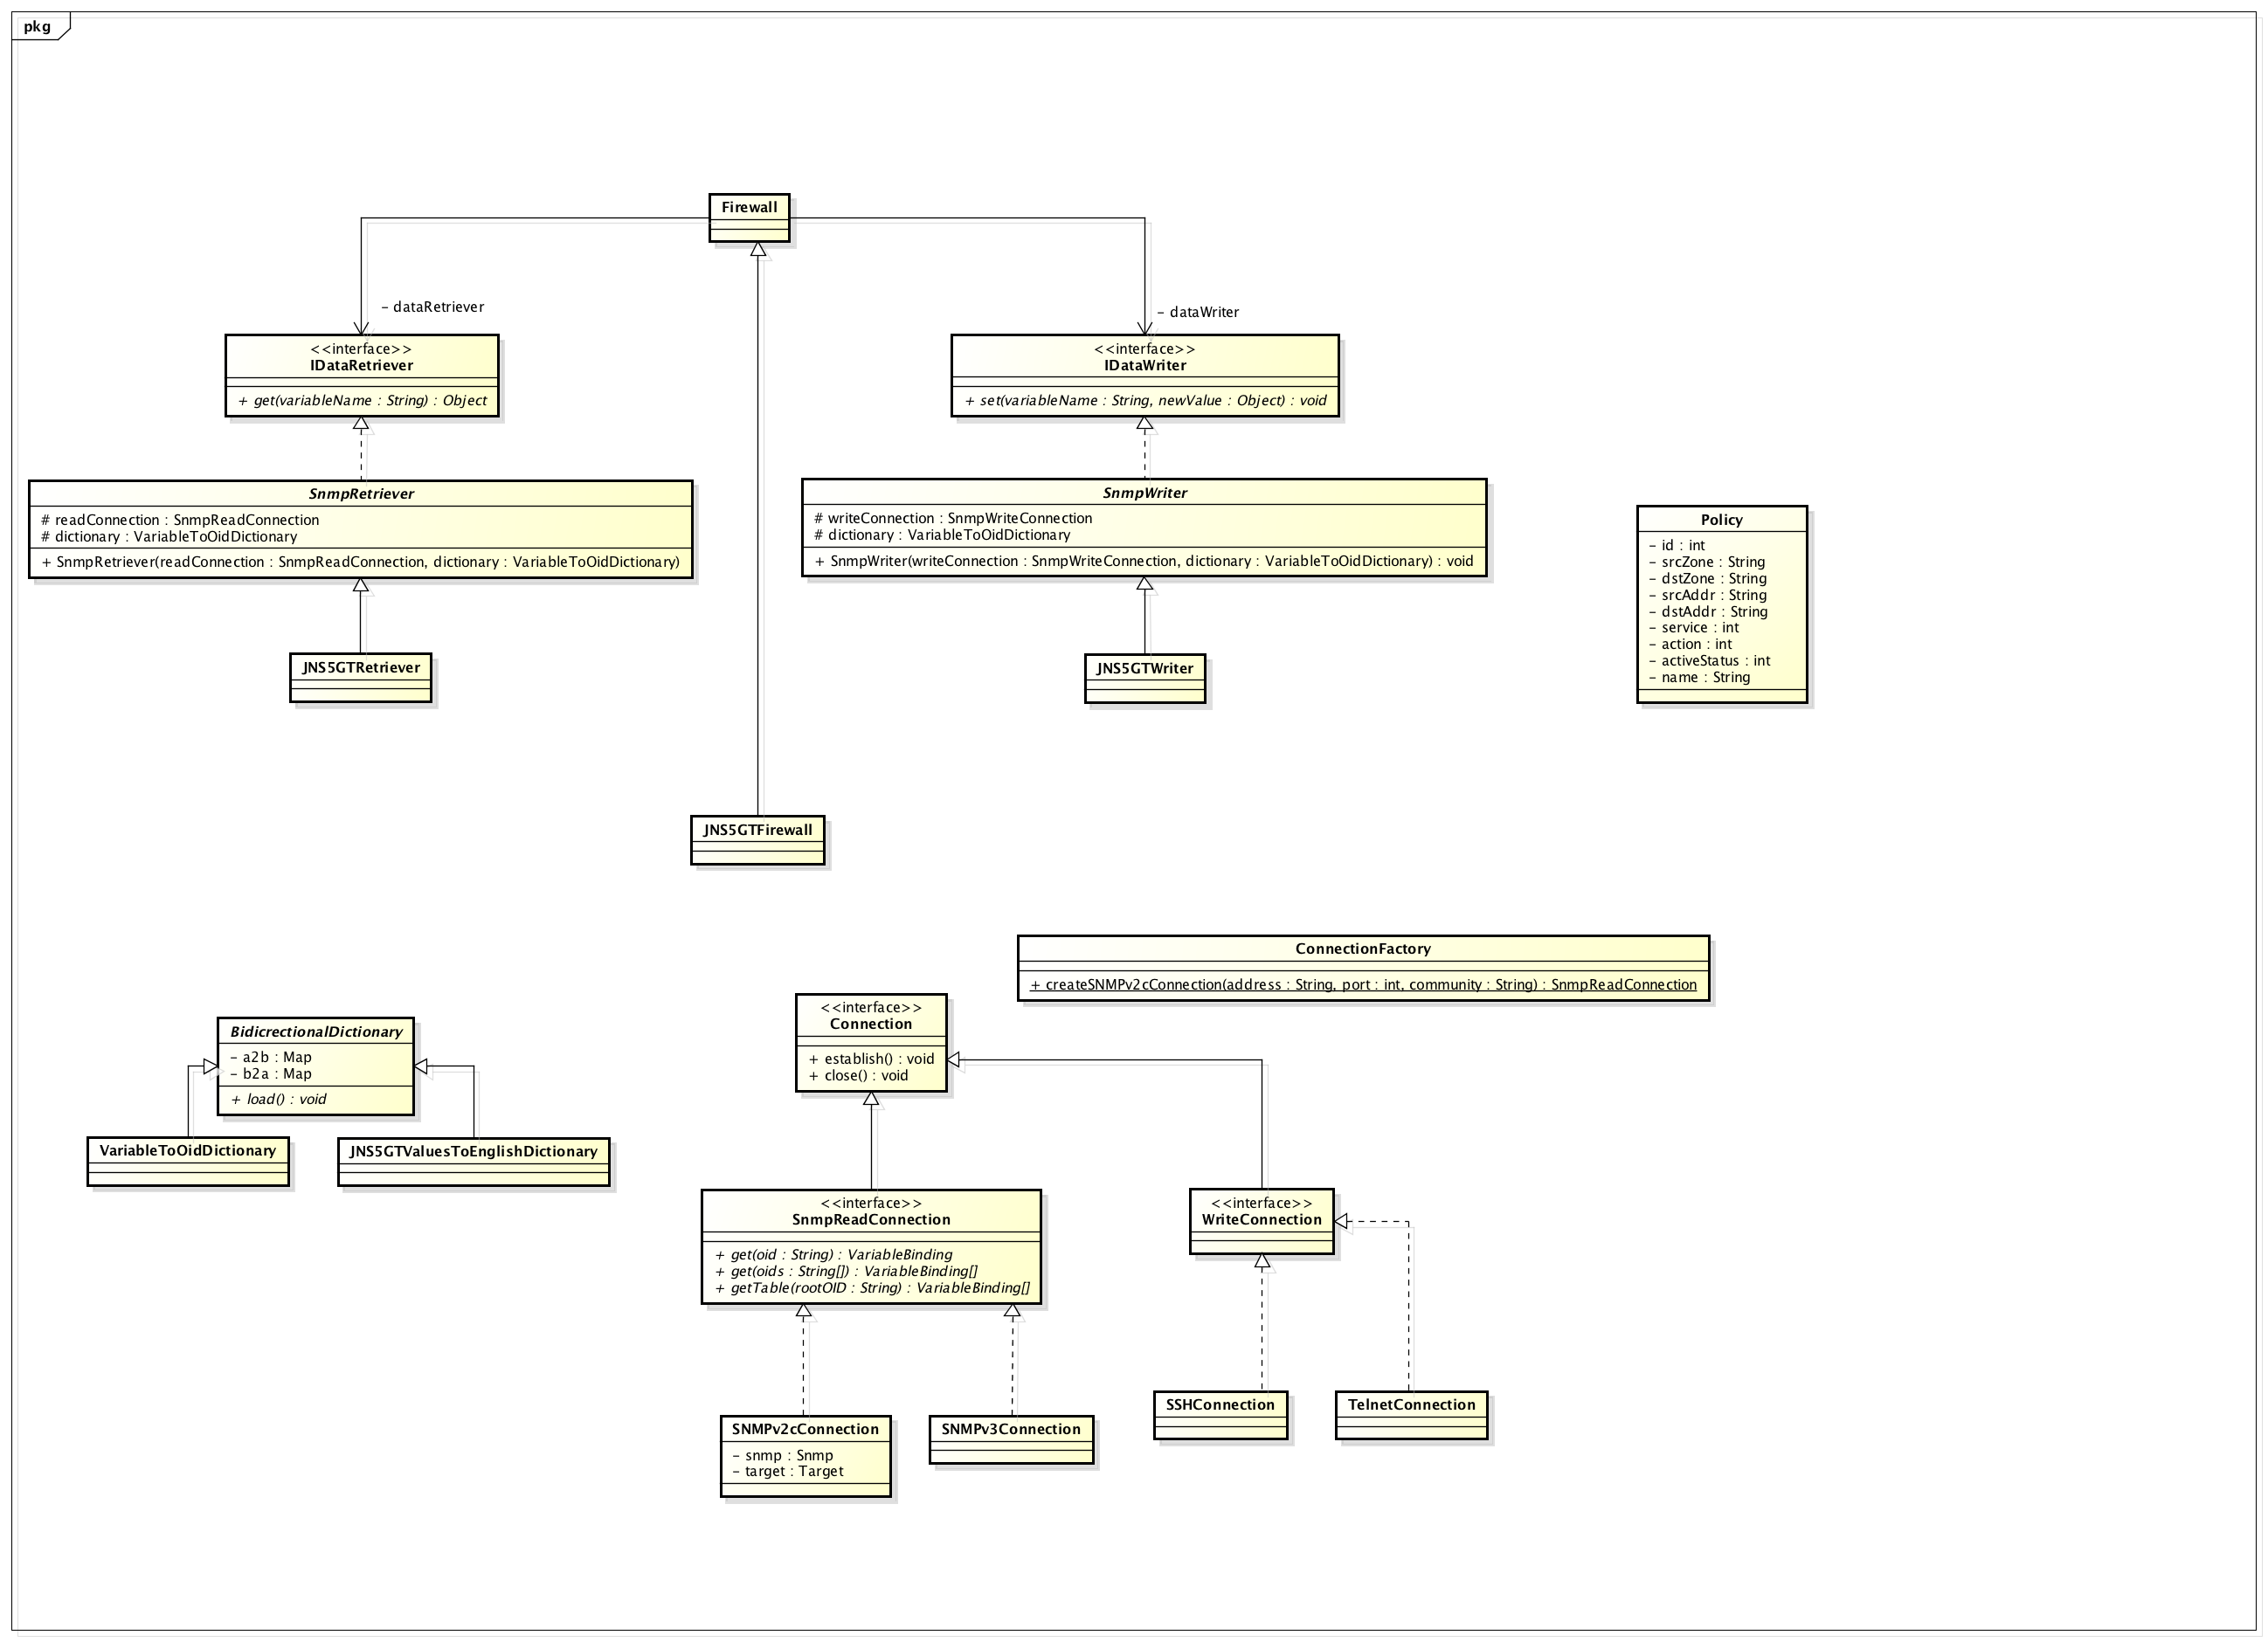
\includegraphics[width=\textwidth]{images/uml}
 
\section{Effort estimation}

\subsection{Basic Tasks}
\begin{tabular} {| l | l | l | l |} \hline
Task &	Original Estimate & Remaining Estimate & Time spent \\ \hline
Preparation for the Tasks &	20 &	0.00 & 24.50 \\ \hline
Listing firewall rules &	7 &	2 &	9.50 \\ \hline
Refreshing rules &	6 &	6 &	0.00 \\ \hline
Visualize thru put & 8 &	4 &	5.00 \\ \hline
Encapsulate the data retrieval &	4	& 0.00 &	4.00 \\ \hline
GUI	 & 10 &	7 &	8.00 \\ \hline
Final Documentation  &	8	& 2	& 5.00 \\ \hline
Basic Total	& 63 &	31.00 &	56.00 \\ \hline
\end{tabular}
\subsection{Advanced Tasks}
\begin{tabular} {| l | l | l | l |}\hline
Task &	Original Estimate & Remaining Estimate & Time spent \\ \hline
Alarm the user &	7	& 5	& 0 \\ \hline
Firewall rules CRUD &	6 &	8 & 	0 \\ \hline
Transactions by Multicast &	8 &	15 &	0 \\ \hline
Exchangeable & 5 & 0	 & 2 \\ \hline
Advanced Total & 26 &	28 &	2 \\ \hline
\end{tabular}

\subsection{Total}
\begin{description}
	\item[Original Estimate]: 89
	\item[Remaining Estimate]: 31
	\item[Time Spent]: 58
\end{description}

\section{Installation}

\section{Technologies}
\subsection{Mock-Objects}
\subsubsection{Setup}

\begin{enumerate}
	\item Download \textit{Mockito} from [1]
	\item Add \textit{junit-4.11.jar} and \textit{mockito-all-1.9.5.jar} to the project's \textit{classpath}
	\item Done
\end{enumerate}

\subsubsection{How to use Mockito}

\textit{Mockito} allows you to mock interfaces, but also concrete classes, with a single line of code:
	
\begin{lstlisting} 
List mockedList = mock(List.class); // creates a mock-Object of `List` 
\end{lstlisting}
	
A \textit{Mockito-Mock-Objects} remembers all methods, which have been called. So you can check afterwards if some method has been called with some parameters.
	
\begin{lstlisting}
	mockedList.add("one");
	    
	verify(mockedList).add("one"); // test "successful" because that exact method with that exact parameter has been called before
	verify(mockedList).add("two"); // test "failed" because `.add("two")` has not been called before
\end{lstlisting}

One of the main functionalities of a Mock-object is that it can provide kind of dummy-methods, called *stubs*, i.e. when a specific method with a specific parameter is called, a specific
value is returned. There are also some kind of wildcards for the methods parameters, if you want to return "first" on any given Integer-parameter. That can be achieved like this:

\begin{lstlisting}
    when(mockedList.get(0)).thenReturn("first"); // `mockedList` will return "first" when `.get(0)` is called
    System.out.println(mockedList.get(0)); // prints "first"
    
    when(mockedList.get(anyInt()).thenReturn("any int"); // will return "any int" if you pass for example: 1, 27, 4, ...
    System.out.println(mockedList.get(2345)); // prints "any int"
\end{lstlisting}

You can also make the mock throw Exceptions by using `.thenThrow()` or make void methods throw Exceptions by:

\begin{lstlisting}
    doThrow(new RuntimeException()).when(mockedList).clear();
    mockedList.clear(); // throws RunTime-Exception
\end{lstlisting}

You can also verify how often a specific method has been called. That works like this:

\begin{lstlisting}
    mockedList.add("once");
    
    verify(mockedList, times(1)).add("once"); // success because `.add("once")` has been called exactly once
    verify(mockedList, times(2)).add("once"); // fails because it has only been called once
\end{lstlisting}

For \textit{times(0)}, you should better use \textit{never()}.
 
Like the number of invocations, you can also verify the order of of invocations:

\begin{lstlisting}
    mockedList.add("first");
    mockedList.add("second");
    
    InOrder inOrder = inOrder(mockedList);
    
    inOrder.verify(mockedList).add("first");
    inOrder.verify(mockedList).add("second");  
\end{lstlisting} 
    
For explanation of additional functionalities and full documentation, see [2].

\subsection{Java FX}
\subsection{SNMP}
\subsubsection{Connection}
\subsubsection{MIBs}
\subsection{Multicast-Groups}

\section{Test report}
\section{Occurred problems}
\bibliography{protokoll}{}
\bibliographystyle{plain}
\end{document}
